\documentclass[onecolumn, draftclsnofoot,10pt, compsoc]{IEEEtran}
\usepackage{graphicx}
\usepackage[section]{placeins}
\usepackage{url}
\usepackage{setspace}

\usepackage{alltt}                                           
\usepackage{float}
\usepackage{color}
\usepackage{url}

\usepackage{geometry}
\geometry{textheight=9.5in, textwidth=7in}
\setlength\parindent{0pt}

% 1. Fill in these details
\def \CapstoneTeamName{\textbf{Insert Team Name Here} }
\def \CapstoneTeamNumber{8}
\def \GroupMemberOne{James Stallkamp}
\def \GroupMemberTwo{Jeremy Fischer}
\def \GroupMemberThree{Austin Row}
\def \CapstoneProjectName{NLP For Digital Manufacturing}
\def \CapstoneSponsorCompany{Autodesk}
\def \CapstoneSponsorPerson{Patti Vrobel}
\def \botname{Aviato }
\def \totalMemoryRequirement{20 MB }

% 2. Uncomment the appropriate line below so that the document type works
\def \DocType{		%Problem Statement
				Requirements Document
				%Technology Review
				%Design Document
				%Progress Report
				}
			
\newcommand{\NameSigPair}[1]{\par
\makebox[2.75in][r]{#1} \hfil 	\makebox[3.25in]{\makebox[2.25in]{\hrulefill} \hfill		\makebox[.75in]{\hrulefill}}
\par\vspace{-12pt} \textit{\tiny\noindent
\makebox[2.75in]{} \hfil		\makebox[3.25in]{\makebox[2.25in][r]{Signature} \hfill	\makebox[.75in][r]{Date}}}}
% 3. If the document is not to be signed, uncomment the RENEWcommand below
\renewcommand{\NameSigPair}[1]{#1}

%%%%%%%%%%%%%%%%%%%%%%%%%%%%%%%%%%%%%%%
\begin{document}
\begin{titlepage}
    \pagenumbering{gobble}
    \begin{singlespace}
    	
\includegraphics[height=4cm]{coe_v_spot1}
        %\hfill 
        % 4. If you have a logo, use this includegraphics command to put it on the coversheet.
        
\includegraphics[height=4cm]{autodesk}   
        \par\vspace{.2in}
        \centering
        \scshape{
            \huge CS Capstone \DocType \par
            {\large\today}\par
            \vspace{.5in}
            \textbf{\Huge\CapstoneProjectName}\par
            \vfill
            {\large Prepared for}\par
            \Huge \CapstoneSponsorCompany\par
            \vspace{5pt}
            {\Large\NameSigPair{\CapstoneSponsorPerson}\par}
            {\large Prepared by }\par
            Group\CapstoneTeamNumber\par
            % 5. comment out the line below this one if you do not wish to name your team
            %\CapstoneTeamName\par 
            \vspace{5pt}
            {\Large
                \NameSigPair{\GroupMemberOne}\par
                \NameSigPair{\GroupMemberTwo}\par
                \NameSigPair{\GroupMemberThree}\par
            }
            \vspace{20pt}
        }
        \begin{abstract}
       		This document outlines the technical requirements of \botname that \CapstoneProjectName must meet. This document starts with an overall description of the project followed by specific functional and performance requirements and ends with a Gantt chart which gives a rough timeline of when each major requirement shall be done.
        \end{abstract}     
    \end{singlespace}
\end{titlepage}
\newpage
\pagenumbering{arabic}
\tableofcontents
% 7. uncomment this (if applicable). Consider adding a page break.
%\listoffigures
%\listoftables
\clearpage

% 8. now you write!
\section{Introduction}
        The introduction outlines the purpose and scope of the project. 
        This section is responsible for defining any prerequisite acronyms and terms used in the document. 
    \subsection{Purpose}
        The purpose of this document is to lay out the requirements of \CapstoneTeamName. 
        This document is a mutual agreement between both parties outlining what will be produced. 
        The intended audience is those who will be working on \CapstoneTeamName and the client for whom \CapstoneTeamName is for.
    \subsection{Scope}
        \botname will be a speech-based virtual assistant for Fusion 360 that lets users perform any one of a subset of tasks within the product, such as saving a document or opening a menu, by verbally instructing it to perform the task.
        Workflows in Fusion 360 that are not suited for handling by a voice interface will not be supported by \botname.
        As a stretch goal, \botname will be capable of questioning user and storing responses to use to predict and automatically assist with future user behavior.
        It will be a plugin that is bundled with Fusion 360 and will be part of the product's standard download.

        \botname will offer users a tool that decreases the time required to achieve their goals within Fusion 360 by offering an interface that runs in parallel with and complements the keyboard and mouse.
        If the stretch goal is achieved, \botname will further increase productivity by learning to predict and automate specific workflows within the product.
        

    \subsection{Definitions, Acronyms, and Abbreviations}
        \begin{table}[h]
            \centering
            \caption{Definitions}
            \label{my-label}
            \begin{tabular}{|l|l|}
                \hline
                \textbf{Term} & \textbf{Definition} \\ \hline
                API & Application programing interface \\ \hline
                CAD & Computer Aided Design \\ \hline
                CAM & Computer Aided Manufacturing \\ \hline
                Fusion 360 & 
                Referred to as just, Fusion, is an Autodesk Cloud-based 3D CAD/CAM tool/product \\ \hline
                Task & In the context of Fusion 360, a function or operation that can be performed in Fusion 360 \\ \hline
                Plugin & Software that adds specific new functionlity to another piece of software \\ \hline
                User & Someone who interacts \botname  \\ \hline
                Workflow & A sequence of tasks \\ \hline
            \end{tabular}
        \end{table}
    %\subsection{References}
        %TODO
    \subsection{Overview}
        %This section describes the contents and organization of the rest of the document. 
        The rest of this document contains a user story outlining intended uses and specific functionalities of \botname as well as assumptions, dependencies, and design constraints. 

\section{Overall Description}
    \subsection{Product Perspective}

        %\subsubsection{System Interfaces}
            %TODO: Revisit this. I'm not sure if it is applicable to this project.
        \subsubsection{User Interfaces}
            The user will interact with \botname via voice commands spoken in English. 
            Therefore to be supported, a device must have a mic.
            In the case of the stretch goal, \botname will periodically speak back to the user to receive insights into the user's actions.

        \subsubsection{Hardware Interfaces} %Included above in the User Interfaces section
            \botname should be supported on desktop and laptop computers that support Fusion 360 and have microphones to receive the user's speech.
            For stretch goal support, devices will also need speakers through which \botname can speak back to the user.
            %TODO: Any other devices? Is there anything else that supports Fusion?

        \subsubsection{Software Interfaces}               
            %TODO: Should the API version/specific open source projects being used be added here?
            \botname needs to translate supported speech commands received from the user to the equivalent tasks within the user's Fusion project.
            The Fusion source code will not be available for modification, thus the commands will need to be executed via the existing Fusion API.
            To translate the commands, the audio recorded by the user interface will need to be processed by a speech-to-text application.
            The resulting output will need to be parsed a another application that can derive meaning from natural language text.
            Finally, the derived meaning will need to have a deterministic mapping to a Fusion API call and thus to a specific task inside of Fusion.
            %TODO: Insert block diagram here.
            %TODO: Describe software interfaces for stretch goal where UI communicates back to user then stores/uses responses
        %\subsubsection{Communications Interfaces}                

        \subsubsection{Memory} 
            \botname should require at most \totalMemoryRequirement of memory to perform the work necessary to add its functionality to Fusion.
            For the stretch goal of storing data related to user responses to questions from \botname, there are no memory caps at this time on the amount of data that can be stored.

        %\subsubsection{Operations}
                %TODO: I'm not sure what this section means.

        \subsubsection{Site Adaptation Requirements} 
            Since \botname interacts with Fusion 360 using existing architecture, Fusion will not need to be modified to support it. 

    \subsection{Product Functions}
		\botname will provide a natural language interface for users, this allows the user to perform many tasks through verbal commands.
		The variety of commmands is large and some examples are saving items, extrude items, or rotating the camera view.
		These voice commands will allow the user to control Fusion360 to the
		
		\botname will periodically ask the users questions regarding the operations they execute.
		In order to start an interview \botname must be able to first recognize a situation where it should be asking a question.
		Then \botname will have to compile a question from infromation mined from the context of the operation in question.
		Once \botname has figured out what to ask it, it must then be able to articule that question into speech.
		For this workflow to create anything useful, the response from the user must be saved for future use.
		\botname will  record user responses and save a transcript along with conextual information.
		The responses to these questions will be used to train \botname to become an intelligent virtual assitant.
		
    \subsection{User Characteristics}
		\botname will have two types of users administrators and, designers. 
		Administrators will have special access to \botname that allows them to perform maintaince.
		\botname must be trained and maintained in order for it to understand different articulations of words and phrases. 
		This maintaince will be in the form of training exercises where administrators will speak with \botname and provide feedback to the system.
		
		The primary and intended user is the designers whom are using Fusion360. 
		Designers building things using Fusion will also be the primary users for \botname.
		Fusion360 users are trying to design or build somthing and as such are more likely to be technically oriented.
		however the software is widely available, so the user could technically be simply anyone who has access to Fusion360.
		At the moment \botname will be designed only to work with Fusion meaning \botname is limited to only Fusion360 users. 

    \subsection{Constraints}
		\botname will be constrained by the API provided by Fusion360. \botname is a plugin for Fusion360 that means \botname will be limited to the API that Fusion360 has made available. 

    \subsection{Assumptions and Dependencies}


\section{Specific Requirements}
    \subsection{External Interface}
    \subsection{Functional Requirements}
    This section includes the requirements that specify all the fundamental actions of the software system.
    	\subsubsection{Functional Requirement 1}
        TITLE: Convert voice to text \\
        DESCRIPTION: The system shall be able to hear voice english statements and output their english text equivalent.
        RATIONAL: This must be done to understand the user's command 
        
        \subsubsection{Functional Requirement 2}
        TITLE: Error State \\
        DESCRIPTION: The system shall inform the user that it can't perform an operation or doesn't understand what the user's commanded is in an error state \\
        RATIONAL: This must be done to inform the user 
        
        \subsubsection{Functional Requirement 3}
        TITLE: Correspond voice command to Fusion 360 action  \\
        DESCRIPTION: The system shall be able to correspond the produced text equivalent described in FR1 to the correct Fusion action
        RATIONAL: This must be done to run commands in Fusion 
        
        \subsubsection{Functional Requirement 4}
        TITLE: Send commands to Fusion  \\
        DESCRIPTION: The system shall be able to send the generated action from FR2 to Fusion
        RATIONAL: This is the last step in the voice command to Fusion action pipeline 
        
        \subsubsection{Functional Requirement 5}
        TITLE: Extrude shape by voice \\
        DESCRIPTION: The system shall be able to extrude a shape accordingly in Fusion by a command similar to "extrude by 5mm."
        RATIONAL: This is the first step in prototype demo 
        
        \subsubsection{Functional Requirement 6}
        TITLE: Rotate camera by voice \\
        DESCRIPTION: The system shall be able to rotate the Fusion camera by a command similar to "rotate the design 90 degrees to the left." 
        RATIONAL: This is the second step in prototype demo 
        
        \subsubsection{Functional Requirement 7}
        TITLE: Save design by voice \\
        DESCRIPTION: The system shall be able to save a Fusion design by a voice command similar to "save my design as \textit{my\_draft\_1.f3d}."
        RATIONAL: This is the last step in prototype demo 
        
        \subsubsection{Functional Requirement 8}
        TITLE: Log file \\
        DESCRIPTION: The system shall store a log file of every attempted command along with if the command was successfully executed or not.
        RATIONAL: This must be done for debugging purposes, and for the exploration of future features.
        
        
        %	%
        %	Below are stretch goals
        %	%
        
        \subsubsection{Stretch Functional Requirement 1}
        TITLE: What interview question to ask \\
        DESCRIPTION: The system shall be able to generate an interview question
        RATIONAL: This is the first step in collecting user reasoning data. 
        
        
        \subsubsection{Stretch Functional Requirement 2}
        TITLE: When to ask an interview question \\
        DESCRIPTION: The system shall be aware of when it is appropriate to ask a question.
        RATIONAL: This is the second step in collecting user reasoning data. 
        
        \subsubsection{Stretch Functional Requirement 3}
        TITLE: Ask a question \\
        DESCRIPTION: The system shall be able to ask a question to the user.
        RATIONAL: This is the third step in collecting user reasoning data. 
        
        \subsubsection{Stretch Functional Requirement 4}
        TITLE: Output interview text to a file \\
        DESCRIPTION: The system shall be able to output an interview question paired with the user's answer to a file.
        RATIONAL: This is the last step in collecting user reasoning data. 
        

   		 \subsection{Performance Requirements}
    		The section covers the numerical performance requirements of the system
        
        \subsubsection{Performance Requirement 1}
        TITLE: Number  of users \\
        DESCRIPTION: \botname can handle one user at time
        RATIONAL: Only one user is using the Fusion at a time. 
        
        \subsubsection{Performance Requirement 2}
        TITLE: Voice command to Fusion action time \\
        DESCRIPTION: A Fusion action shall take place within one a second of the user's voice command.
        RATIONAL: This window is fast enough for a user's satisfaction and slow enough to allow \botname to process fully.
        
        \subsubsection{Performance Requirement 3}
        TITLE: Number  of users \\
        DESCRIPTION: \botname can handle one user at time
        RATIONAL: Only one user is using the Fusion at a time. 
        
    \subsection{Design Constraints}
    	\CapstoneTeamName doesn't have access to the Fusion source code. Therefore, \CapstoneTeamName is constrained by the depth and breadth of the Fusion API in the creation of \botname.
        
    \subsection{Software System Attributes}
	   	\subsubsection{Reliability}
	   	SCALE: The desired task is performed, i.e. if \botname is capable of performing the desired action then it shall be able to understand the voice command and successfully execute the Fusion action.\\
	   	METER: Measurements obtained from 10 trials per possible command during testing.\\
	   	MUST: More than 75\% of achievable voice commands.\\
	   	PLAN: More than 80\% of achievable voice commands.\\
	   	WISH: 90\% of achievable voice commands.\\
   
		

\section{Release Plan}
	The develop of \botname is very sequential. Each step's development and success depends on how the previous step was implemented. For that reason, \CapstoneProjectName's release plan remains tentative. Below is a Gantt chart outlining \botname's development plan.
    \subsection{Release plan}
    	\begin{figure}[H]
    		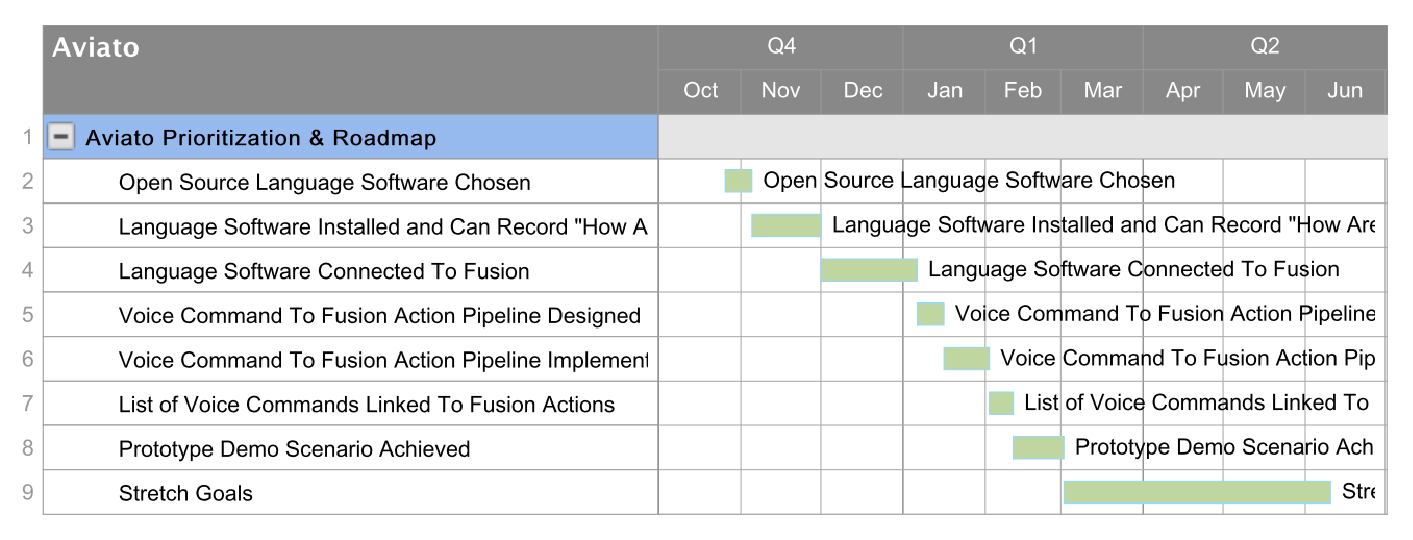
\includegraphics[width=1\textwidth]{ganttChart.eps}
    		\centering
    		\caption{Gantt chart describing \CapstoneProjectName's tentative development schedule}
   			\label{fig:mesh1}
    	\end{figure}


%\bibliography{requirementsBib} 
%\bibliographystyle{ieeetr}

\end{document}
